% Choose one to switch between slides and handout
\documentclass[]{beamer}
%\documentclass[handout]{beamer}

% Video Meta Data
\title{Bitcoin, Blockchain and Cryptoassets}
\subtitle{Payment Channels and Lightning Network}
\author{Prof. Dr. Fabian Schär}
\institute{University of Basel}

% Config File
% Packages
\usepackage[utf8]{inputenc}
\usepackage{hyperref}
\usepackage{gitinfo2}
\usepackage{tikz}
\usepackage{amsmath}
\usepackage{mathtools}
\usepackage{bibentry}
\usepackage{xcolor}
\usepackage{colortbl} % Add colour to LaTeX tables
\usepackage{caption}
\usepackage[export]{adjustbox}
\usepackage{pgfplots} \pgfplotsset{compat = 1.17}
\usepackage{makecell}
\usepackage{fancybox}
\usepackage{ragged2e}
\usepackage{fontawesome}
\usepackage{seqsplit}
\usepackage{tabularx}

% Color Options
\definecolor{highlight}{rgb}{0.65,0.84,0.82}
\definecolor{focus}{rgb}{0.72, 0, 0}
\definecolor{lightred}{rgb}{0.8,0.5,0.5}
\definecolor{midgray}{RGB}{190,195,200}

% Beamer Template Options
\beamertemplatenavigationsymbolsempty
\setbeamertemplate{footline}[frame number]
\setbeamercolor{structure}{fg=black}
\setbeamercolor{footline}{fg=black}
\setbeamercolor{title}{fg=black}
\setbeamercolor{frametitle}{fg=black}
\setbeamercolor{item}{fg=black}
\setbeamercolor{}{fg=black}
\setbeamercolor{bibliography item}{fg=black}
\setbeamercolor*{bibliography entry title}{fg=black}
\setbeamercolor{alerted text}{fg=focus}
\setbeamertemplate{items}[square]
\setbeamertemplate{enumerate items}[default]
\captionsetup[figure]{labelfont={color=black},font={color=black}}
\captionsetup[table]{labelfont={color=black},font={color=black}}

\setbeamertemplate{bibliography item}{\insertbiblabel}

% Link Icon Command
\newcommand{\link}{%
    \tikz[x=1.2ex, y=1.2ex, baseline=-0.05ex]{%
        \begin{scope}[x=1ex, y=1ex]
            \clip (-0.1,-0.1)
                --++ (-0, 1.2)
                --++ (0.6, 0)
                --++ (0, -0.6)
                --++ (0.6, 0)
                --++ (0, -1);
            \path[draw,
                line width = 0.5,
                rounded corners=0.5]
                (0,0) rectangle (1,1);
        \end{scope}
        \path[draw, line width = 0.5] (0.5, 0.5)
            -- (1, 1);
        \path[draw, line width = 0.5] (0.6, 1)
            -- (1, 1) -- (1, 0.6);
        }
    }

% Read Git Data from Github Actions Workflow
% Defaults to gitinfo2 for local builds
\IfFileExists{gitInfo.txt}
	{\input{gitInfo.txt}}
	{
		\newcommand{\gitRelease}{(Local Release)}
		\newcommand{\gitSHA}{\gitHash}
		\newcommand{\gitDate}{\gitAuthorIsoDate}
	}

% Custom Titlepage
\defbeamertemplate*{title page}{customized}[1][]
{
  \vspace{-0cm}\hfill\includegraphics[width=2.5cm]{../config/logo_cif}
  \includegraphics[width=1.9cm]{../config/seal_wwz}
  \\ \vspace{2em}
  \usebeamerfont{title}\textbf{\inserttitle}\par
  \usebeamerfont{title}\usebeamercolor[fg]{title}\insertsubtitle\par  \vspace{1.5em}
  \small\usebeamerfont{author}\insertauthor\par
  \usebeamerfont{author}\insertinstitute\par \vspace{2em}
  \usebeamercolor[fg]{titlegraphic}\inserttitlegraphic
    \tiny \noindent \texttt{Release Ver.: \gitRelease}\\ 
    \texttt{Version Hash: \gitSHA}\\
    \texttt{Version Date: \gitDate}\\ \vspace{1em}
    
    
    \iffalse
  \link \href{https://github.com/cifunibas/Bitcoin-Blockchain-Cryptoassets/blob/main/slides/intro.pdf}
  {Get most recent version}\\
  \link \href{https://github.com/cifunibas/Bitcoin-Blockchain-Cryptoassets/blob/main/slides/intro.pdf}
  {Watch video lecture}\\ 
  
  \fi
  
  \vspace{1em}
  License: \texttt{Creative Commons Attribution-NonCommercial-ShareAlike 4.0 International}\\\vspace{2em}
  \includegraphics[width = 1.2cm]{../config/license}
}


% tikzlibraries
\usetikzlibrary{decorations.pathreplacing}
\usetikzlibrary{decorations.markings}
\usetikzlibrary{positioning}
\usetikzlibrary{calc}
\captionsetup{font=footnotesize}


%%%%%%%%%%%%%%%%%%%%%%%%%%%%%%%%%%%%%%%%%%%%%%
%%%%%%%%%%%%%%%%%%%%%%%%%%%%%%%%%%%%%%%%%%%%%%
\begin{document}

\thispagestyle{empty}
\begin{frame}[noframenumbering]
	\titlepage
\end{frame}
%%%

%%%
\begin{frame}{Basic Idea of State Channels}

What we know already:
\begin{itemize}
	\item The Bitcoin network today is facing scalability challenges.\ \textit{Block cadence or size increase are cannot solve this.}
	\item Economic scripting, i.e., the clever combination of transaction designs and conditions, allows to account for different incentive scenarios in the context of transactions.
\end{itemize}

\vspace{1.5 em}

\uncover<2->{
\textbf{State channels} present another scalability option, reducing the transaction load on the network between two agents that exchange payments frequently:

\begin{itemize}
	\item Establishment and funding of payment channel.
	\item Off-chain transaction handling between the two participants.
	\item Channel closure with net settling of transactions on-chain.
\end{itemize}
}

\end{frame}
%%%

%%%
\begin{frame}{A Naïve Implementation}


\end{frame}
%%%


%%%
\begin{frame}{Unidirectional Payment Channel (UPC): Setup}
\begin{minipage}{0.1\linewidth}
		\vspace{-0.5cm}
		\centering
		
\includegraphics[width=1cm]{../assets/images/agents/handing_right}
		\\ \hspace{-0.35cm} \textbf{Alice}
	\end{minipage}%
	\begin{minipage}{0.8\linewidth}
		\begin{figure}
		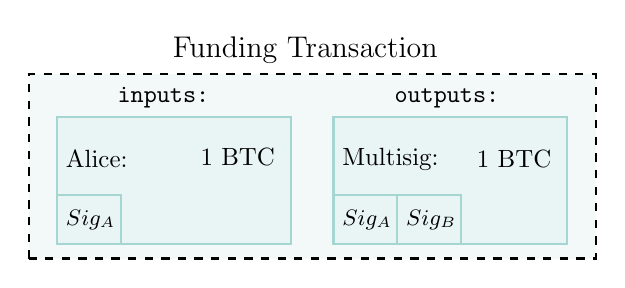
\begin{tikzpicture}[scale=0.9, every node/.style={scale=0.9}]
			
	\filldraw[yshift=-0.05cm, xshift=0.1cm,color = highlight!15, thick, 	draw=black, dashed] (-3,-3.6) rectangle ++(8cm,2.6cm);
	
	\draw[color=black] plot (1,-0.4) node [below]
	{\large{{Funding Transaction}}};
	
	% Inputs
	\draw[color=black] plot (-1,-1.65) node[above] {\texttt{inputs:}};
	
	% top left
	\filldraw[yshift=-0.05cm, xshift=0.1cm,color = highlight!25, thick, 	draw=highlight] (-2.6,-3.4) rectangle ++(3.3cm,1.8cm);
	\filldraw[yshift=-0.05cm, xshift=0.1cm,color = highlight!25, thick, 	draw=highlight] (-2.6,-3.4) rectangle ++(0.9cm,0.7cm);
	\draw[color=black] plot (-2.5,-2.25) node[right] {Alice:};
	\draw[color=black] plot (-0.6,-2.21)   node[right] {1 BTC};
	\draw[color=black] plot (-2.5,-3.1)   node[right] {\small{$Sig_A$}};
	
	\draw plot (-2,-3.1) node {\checkmarkgreen};
	
	% Outputs
	\draw[color=black] plot (3,-1.65)   node[above] {\texttt{outputs:}};
	
	% top right
	\filldraw[yshift=-0.05cm, xshift=0.1cm,color = highlight!25, thick, draw=highlight] (1.3,-3.4) rectangle ++(3.3cm,1.8cm);
	\filldraw[yshift=-0.05cm, xshift=0.1cm,color = highlight!25, thick, 	draw=highlight] (1.3,-3.4) rectangle ++(0.9cm,0.7cm);
	\filldraw[yshift=-0.05cm, xshift=0.1cm,color = highlight!25, thick, 	draw=highlight] (2.2,-3.4) rectangle ++(0.9cm,0.7cm);
	\draw[color=black] plot (1.4,-2.25)   node[right] {Multisig:};
	\draw[color=black] plot (3.3,-2.25)   node[right] {1 BTC};
	\draw[color=black] plot (1.4,-3.1)   node[right] {\small{$Sig_A$}};
	\draw[color=black] plot (2.3,-3.1)   node[right] {\small{$Sig_B$}};

		\end{tikzpicture}
		\vspace{0.5cm}
		\uncover<2 ->{
		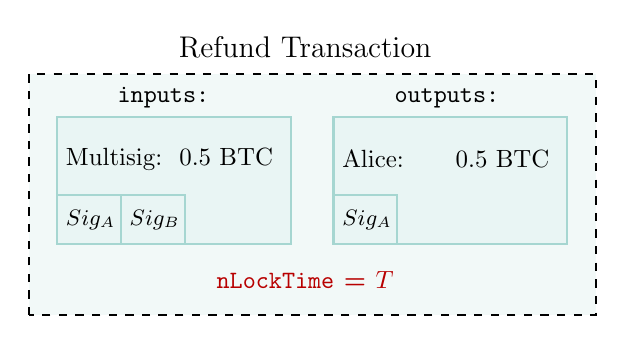
\begin{tikzpicture}[scale=0.9, every node/.style={scale=0.9}]
				\filldraw[yshift=-0.05cm, xshift=0.1cm,color = highlight!15, thick, 	draw=black, dashed] (-3,-4.4) rectangle ++(8cm,3.4cm);
	
	\draw[color=black] plot (1,-0.4) node [below]
	{\large{{Refund Transaction}}};
	
	% Inputs
	\draw[color=black] plot (-1,-1.65) node[above] {\texttt{inputs:}};
	
	% top left
	\filldraw[yshift=-0.05cm, xshift=0.1cm,color = highlight!25, thick, 	draw=highlight] (-2.6,-3.4) rectangle ++(3.3cm,1.8cm);
	\filldraw[yshift=-0.05cm, xshift=0.1cm,color = highlight!25, thick, 	draw=highlight] (-2.6,-3.4) rectangle 	++(0.9cm,0.7cm);
	\filldraw[yshift=-0.05cm, xshift=0.1cm,color = highlight!25, thick, 	draw=highlight] (-1.7,-3.4) rectangle 	++(0.9cm,0.7cm);
	\draw[color=black] plot (-2.5,-2.25) node[right] {Multisig:};
	\draw[color=black] plot (-0.9,-2.21)   node[right] {0.5 BTC};
	\draw[color=black] plot (-2.5,-3.1)   node[right] {\small{$Sig_A$}};
	\draw[color=black] plot (-1.6,-3.1)   node[right] {\small{$Sig_B$}};
	
	\draw plot (-1.1,-3.1) node {\checkmarkgreen};
	
	% Outputs
	\draw[color=black] plot (3,-1.65)   node[above] {\texttt{outputs:}};
	
	% top right
	\filldraw[yshift=-0.05cm, xshift=0.1cm,color = highlight!25, thick, draw=highlight] (1.3,-3.4) rectangle ++(3.3cm,1.8cm);
	\filldraw[yshift=-0.05cm, xshift=0.1cm,color = highlight!25, thick, 	draw=highlight] (1.3,-3.4) rectangle ++(0.9cm,0.7cm);
	\draw[color=black] plot (1.4,-2.25)   node[right] {Alice:};
	\draw[color=black] plot (3,-2.25)   node[right] {0.5 BTC};
	\draw[color=black] plot (1.4,-3.1)   node[right] {\small{$Sig_A$}};
	
	% Time lock
	\draw[color=focus] plot (1,-4.2)   node[above] {\textbf{\texttt{nLockTime} = $T$}};

		\end{tikzpicture}
		}
		\end{figure}
	\end{minipage}%
	\begin{minipage}{0.1\linewidth}
		\vspace{-0.5cm}
		\centering
		
\includegraphics[width=1cm]{../assets/images/agents/handing_left}
		\\ \hspace{0.3cm}\textbf{Bob}
	\end{minipage}

\end{frame}
%%%

%%%
\begin{frame}{UPC: Exchanging Payments}
\begin{minipage}{0.1\linewidth}
		\vspace{-2.1cm}
		\begin{figure}[t]
			\resizebox{2.5cm}{!}{
			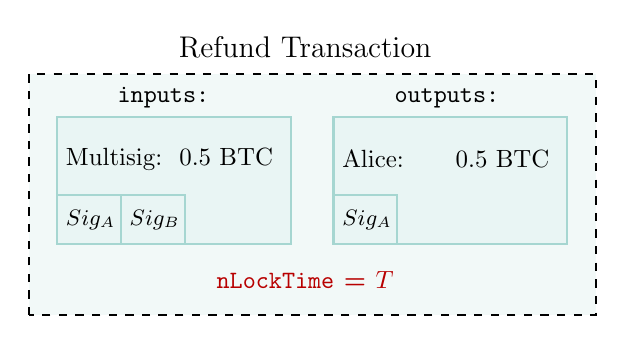
\begin{tikzpicture}[scale=0.9, every node/.style={scale=0.9}]
						\filldraw[yshift=-0.05cm, xshift=0.1cm,color = highlight!15, thick, 	draw=black, dashed] (-3,-4.4) rectangle ++(8cm,3.4cm);
	
	\draw[color=black] plot (1,-0.4) node [below]
	{\large{{Refund Transaction}}};
	
	% Inputs
	\draw[color=black] plot (-1,-1.65) node[above] {\texttt{inputs:}};
	
	% top left
	\filldraw[yshift=-0.05cm, xshift=0.1cm,color = highlight!25, thick, 	draw=highlight] (-2.6,-3.4) rectangle ++(3.3cm,1.8cm);
	\filldraw[yshift=-0.05cm, xshift=0.1cm,color = highlight!25, thick, 	draw=highlight] (-2.6,-3.4) rectangle 	++(0.9cm,0.7cm);
	\filldraw[yshift=-0.05cm, xshift=0.1cm,color = highlight!25, thick, 	draw=highlight] (-1.7,-3.4) rectangle 	++(0.9cm,0.7cm);
	\draw[color=black] plot (-2.5,-2.25) node[right] {Multisig:};
	\draw[color=black] plot (-0.9,-2.21)   node[right] {0.5 BTC};
	\draw[color=black] plot (-2.5,-3.1)   node[right] {\small{$Sig_A$}};
	\draw[color=black] plot (-1.6,-3.1)   node[right] {\small{$Sig_B$}};
	
	\draw plot (-1.1,-3.1) node {\checkmarkgreen};
	
	% Outputs
	\draw[color=black] plot (3,-1.65)   node[above] {\texttt{outputs:}};
	
	% top right
	\filldraw[yshift=-0.05cm, xshift=0.1cm,color = highlight!25, thick, draw=highlight] (1.3,-3.4) rectangle ++(3.3cm,1.8cm);
	\filldraw[yshift=-0.05cm, xshift=0.1cm,color = highlight!25, thick, 	draw=highlight] (1.3,-3.4) rectangle ++(0.9cm,0.7cm);
	\draw[color=black] plot (1.4,-2.25)   node[right] {Alice:};
	\draw[color=black] plot (3,-2.25)   node[right] {0.5 BTC};
	\draw[color=black] plot (1.4,-3.1)   node[right] {\small{$Sig_A$}};
	
	% Time lock
	\draw[color=focus] plot (1,-4.2)   node[above] {\textbf{\texttt{nLockTime} = $T$}};

			\end{tikzpicture}}
		\end{figure}
		\centering
		
\includegraphics[width=1cm]{../assets/images/agents/handing_right}
		\\ \hspace{-0.35cm} \textbf{Alice}
	\end{minipage}%
	\begin{minipage}{0.8\linewidth}
		\uncover<3->{
		\vspace{1cm}
		\begin{figure}
				\resizebox{5cm}{!}{
					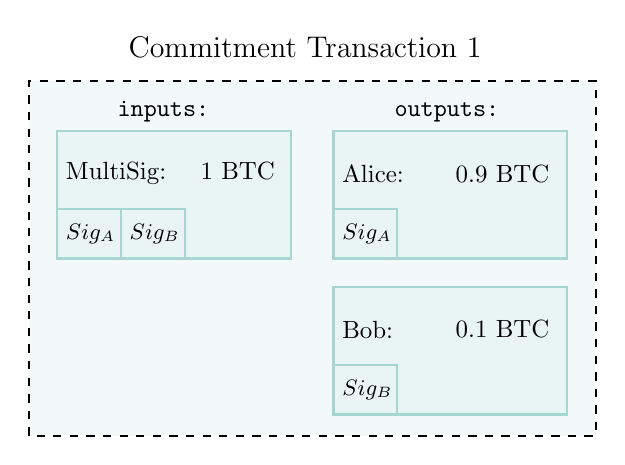
\begin{tikzpicture}[scale=0.9, every node/.style={scale=0.9}]
							\filldraw[yshift=-0.05cm, xshift=0.1cm,color = highlight!15, thick, 	draw=black, dashed] (-3,-5.9) rectangle ++(8cm,5cm);
	
	\draw[color=black] plot (1,-0.2) node [below]
	{\large{{Commitment Transaction 1}}};
	
	% Inputs
	\draw[color=black] plot (-1,-1.65) node[above] {\texttt{inputs:}};
	
	% top left
	\filldraw[yshift=-0.05cm, xshift=0.1cm,color = highlight!25, thick, 	draw=highlight] (-2.6,-3.4) rectangle ++(3.3cm,1.8cm);
	\filldraw[yshift=-0.05cm, xshift=0.1cm,color = highlight!25, thick, 	draw=highlight] (-2.6,-3.4) rectangle ++(0.9cm,0.7cm);
	\filldraw[yshift=-0.05cm, xshift=0.1cm,color = highlight!25, thick, 	draw=highlight] (-1.7,-3.4) rectangle ++(0.9cm,0.7cm);
	\draw[color=black] plot (-2.5,-2.25) node[right] {MultiSig:};
	\draw[color=black] plot (-0.6,-2.21)   node[right] {1 BTC};
	\draw[color=black] plot (-2.5,-3.1)   node[right] {\small{$Sig_A$}};
	\draw[color=black] plot (-1.6,-3.1)   node[right] {\small{$Sig_B$}};
	
	\draw plot (-2,-3.1) node {\checkmarkgreen};
	
	% Outputs
	\draw[color=black] plot (3,-1.65)   node[above] {\texttt{outputs:}};
	
	% top right
	\filldraw[yshift=-0.05cm, xshift=0.1cm,color = highlight!25, thick, draw=highlight] (1.3,-3.4) rectangle ++(3.3cm,1.8cm);
	\filldraw[yshift=-0.05cm, xshift=0.1cm,color = highlight!25, thick, 	draw=highlight] (1.3,-3.4) rectangle ++(0.9cm,0.7cm);
	\draw[color=black] plot (1.4,-2.25)   node[right] {Alice:};
	\draw[color=black] plot (3,-2.25)   node[right] {0.9 BTC};
	\draw[color=black] plot (1.4,-3.1)   node[right] {\small{$Sig_A$}};
	
	% bottom right
	\filldraw[yshift=-0.05cm, xshift=0.1cm,color = highlight!25, thick, draw=highlight] (1.3,-5.6) rectangle ++(3.3cm,1.8cm);
	\filldraw[yshift=-0.05cm, xshift=0.1cm,color = highlight!25, thick,draw=highlight] (1.3,-5.6) rectangle ++(0.9cm,0.7cm);
	\draw[color=black] plot (1.4,-4.45)   node[right] {Bob:};
	\draw[color=black] plot (3,-4.45)   node[right] {0.1 BTC};
	\draw[color=black] plot (1.4,-5.3)   node[right] {\small{$Sig_B$}};

				\end{tikzpicture}}
		\end{figure}}
		\begin{figure}
			\centering
			\resizebox{4cm}{!}{
			\begin{tikzpicture}[scale=1, every node/.style={scale=1}]
					
% Title
%\node[above] at (2,4.3) {Peer-to-Peer};


% Network
\node (agenta) at (1,2.8) {\includegraphics[width = 0.6 cm]{../assets/images/agents/avatar_rand3.png}};
\node (agentb) at (0.5,1) {\includegraphics[width = 0.6 cm]{../assets/images/agents/avatar_rand4.png}};
\node (agentc) at (3,2.1) {\includegraphics[width = 0.6 cm]{../assets/images/agents/avatar_rand5.png}};
\node (agentd) at (2.8,0) {\includegraphics[width = 0.6 cm]{../assets/images/agents/avatar_rand1.png}};
\node (agente) at (5,4.3) {\includegraphics[width = 0.6 cm]{../assets/images/agents/avatar_rand2.png}};	
\node (agentf) at (5.1,1.1) {\includegraphics[width = 0.6 cm]{../assets/images/agents/avatar_rand3.png}};
\node (agentg) at (7.5,3.8) {\includegraphics[width = 0.6 cm]{../assets/images/agents/avatar_rand4.png}};
\node (agenth) at (6.7,0.4) {\includegraphics[width = 0.6 cm]{../assets/images/agents/avatar_rand5.png}};

% Network flow
\draw[<->, thick, dashed]	(agenta.south) -- (agentb.north);
\draw[<->, thick, dashed] 	(agenta.east) -- (agente.west);
\draw[<->, thick, dashed]	(agenta.south east) -- (agentc.west);
\draw[<->, thick, dashed]	(agente.south west) -- (agentc.north east);
\draw[<->, thick, dashed]	(agente.south) -- (agentf.north);
\draw[<->, thick, dashed]	(agente.east) -- (agentg.west);
\draw[<->, thick, dashed]	(agentc.south west) -- (agentb.east);
\draw[<->, thick, dashed]	(agentc.south) -- (agentd.north);
\draw[<->, thick, dashed]	(agentc.south east) --  (agentf.west);
\draw[<->, thick, dashed]	(agentg.south west) -- (agentf.north east);
\draw[<->, thick, dashed]	(agentg.south) -- (agenth.north);
\draw[<->, thick, dashed]	(agentb.south east) -- (agentd.west);
\draw[<->, thick, dashed]	(agentf.south west) -- (agentd.east);
\draw[<->, thick, dashed]	(agentf.south east) -- (agenth.west);
\draw[<->, thick, dashed]	(agenth.south west) -- (agentd.east);

			\end{tikzpicture}}
		\end{figure}
		\uncover<2>{
			\vspace{-2.6cm}
			\begin{figure}
				\resizebox{2.5cm}{!}{
				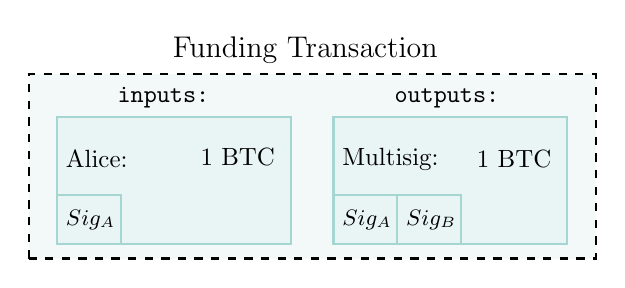
\begin{tikzpicture}[scale=0.9, every node/.style={scale=0.9}]
						
	\filldraw[yshift=-0.05cm, xshift=0.1cm,color = highlight!15, thick, 	draw=black, dashed] (-3,-3.6) rectangle ++(8cm,2.6cm);
	
	\draw[color=black] plot (1,-0.4) node [below]
	{\large{{Funding Transaction}}};
	
	% Inputs
	\draw[color=black] plot (-1,-1.65) node[above] {\texttt{inputs:}};
	
	% top left
	\filldraw[yshift=-0.05cm, xshift=0.1cm,color = highlight!25, thick, 	draw=highlight] (-2.6,-3.4) rectangle ++(3.3cm,1.8cm);
	\filldraw[yshift=-0.05cm, xshift=0.1cm,color = highlight!25, thick, 	draw=highlight] (-2.6,-3.4) rectangle ++(0.9cm,0.7cm);
	\draw[color=black] plot (-2.5,-2.25) node[right] {Alice:};
	\draw[color=black] plot (-0.6,-2.21)   node[right] {1 BTC};
	\draw[color=black] plot (-2.5,-3.1)   node[right] {\small{$Sig_A$}};
	
	\draw plot (-2,-3.1) node {\checkmarkgreen};
	
	% Outputs
	\draw[color=black] plot (3,-1.65)   node[above] {\texttt{outputs:}};
	
	% top right
	\filldraw[yshift=-0.05cm, xshift=0.1cm,color = highlight!25, thick, draw=highlight] (1.3,-3.4) rectangle ++(3.3cm,1.8cm);
	\filldraw[yshift=-0.05cm, xshift=0.1cm,color = highlight!25, thick, 	draw=highlight] (1.3,-3.4) rectangle ++(0.9cm,0.7cm);
	\filldraw[yshift=-0.05cm, xshift=0.1cm,color = highlight!25, thick, 	draw=highlight] (2.2,-3.4) rectangle ++(0.9cm,0.7cm);
	\draw[color=black] plot (1.4,-2.25)   node[right] {Multisig:};
	\draw[color=black] plot (3.3,-2.25)   node[right] {1 BTC};
	\draw[color=black] plot (1.4,-3.1)   node[right] {\small{$Sig_A$}};
	\draw[color=black] plot (2.3,-3.1)   node[right] {\small{$Sig_B$}};

				\end{tikzpicture}}
			\end{figure}
		}		
	\end{minipage}%
	\begin{minipage}{0.1\linewidth}
		\vspace{-0.5cm}
		\centering
		
\includegraphics[width=1cm]{../assets/images/agents/handing_left}
		\\ \hspace{0.3cm}\textbf{Bob}
	\end{minipage}

\end{frame}
%%%

\begin{frame}{Let's see}
	\begin{minipage}{0.1\linewidth}
		\vspace{-2.27cm}
		\begin{figure}[t]
			\resizebox{2.5cm}{!}{
			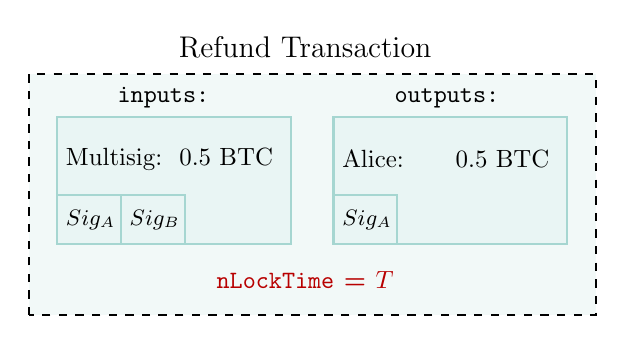
\begin{tikzpicture}[scale=0.9, every node/.style={scale=0.9}]
					\filldraw[yshift=-0.05cm, xshift=0.1cm,color = highlight!15, thick, 	draw=black, dashed] (-3,-4.4) rectangle ++(8cm,3.4cm);
	
	\draw[color=black] plot (1,-0.4) node [below]
	{\large{{Refund Transaction}}};
	
	% Inputs
	\draw[color=black] plot (-1,-1.65) node[above] {\texttt{inputs:}};
	
	% top left
	\filldraw[yshift=-0.05cm, xshift=0.1cm,color = highlight!25, thick, 	draw=highlight] (-2.6,-3.4) rectangle ++(3.3cm,1.8cm);
	\filldraw[yshift=-0.05cm, xshift=0.1cm,color = highlight!25, thick, 	draw=highlight] (-2.6,-3.4) rectangle 	++(0.9cm,0.7cm);
	\filldraw[yshift=-0.05cm, xshift=0.1cm,color = highlight!25, thick, 	draw=highlight] (-1.7,-3.4) rectangle 	++(0.9cm,0.7cm);
	\draw[color=black] plot (-2.5,-2.25) node[right] {Multisig:};
	\draw[color=black] plot (-0.9,-2.21)   node[right] {0.5 BTC};
	\draw[color=black] plot (-2.5,-3.1)   node[right] {\small{$Sig_A$}};
	\draw[color=black] plot (-1.6,-3.1)   node[right] {\small{$Sig_B$}};
	
	\draw plot (-1.1,-3.1) node {\checkmarkgreen};
	
	% Outputs
	\draw[color=black] plot (3,-1.65)   node[above] {\texttt{outputs:}};
	
	% top right
	\filldraw[yshift=-0.05cm, xshift=0.1cm,color = highlight!25, thick, draw=highlight] (1.3,-3.4) rectangle ++(3.3cm,1.8cm);
	\filldraw[yshift=-0.05cm, xshift=0.1cm,color = highlight!25, thick, 	draw=highlight] (1.3,-3.4) rectangle ++(0.9cm,0.7cm);
	\draw[color=black] plot (1.4,-2.25)   node[right] {Alice:};
	\draw[color=black] plot (3,-2.25)   node[right] {0.5 BTC};
	\draw[color=black] plot (1.4,-3.1)   node[right] {\small{$Sig_A$}};
	
	% Time lock
	\draw[color=focus] plot (1,-4.2)   node[above] {\textbf{\texttt{nLockTime} = $T$}};

			\end{tikzpicture}}
		\end{figure}
		\centering
		
\includegraphics[width=1cm]{../assets/images/agents/handing_right}
		\\ \hspace{-0.35cm} \textbf{Alice}
	\end{minipage}%
	\begin{minipage}{0.8\linewidth}
		\vspace{1.34cm}
		\only<1>{
			\begin{figure}
				\resizebox{5cm}{!}{
					\begin{tikzpicture}
						\filldraw[yshift=-0.05cm, xshift=0.1cm,color = white!15, thick, draw=white] (-3,-5.9) rectangle ++(8cm,5.7cm);
				\end{tikzpicture}}
		\end{figure}}
		\only<2-3>{
			\begin{figure}
				\resizebox{5cm}{!}{
				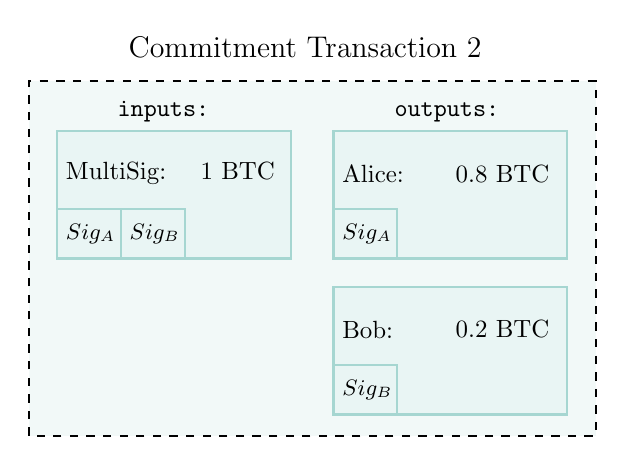
\begin{tikzpicture}[scale=0.9, every node/.style={scale=0.9}]
					\filldraw[yshift=-0.05cm, xshift=0.1cm,color = highlight!15, thick, 	draw=black, dashed] (-3,-5.9) rectangle ++(8cm,5cm);

\draw[color=black] plot (1,-0.2) node [below]
{\large{{Commitment Transaction 2}}};

% Inputs
\draw[color=black] plot (-1,-1.65) node[above] {\texttt{inputs:}};

% top left
\filldraw[yshift=-0.05cm, xshift=0.1cm,color = highlight!25, thick, 	draw=highlight] (-2.6,-3.4) rectangle ++(3.3cm,1.8cm);
\filldraw[yshift=-0.05cm, xshift=0.1cm,color = highlight!25, thick, 	draw=highlight] (-2.6,-3.4) rectangle ++(0.9cm,0.7cm);
\filldraw[yshift=-0.05cm, xshift=0.1cm,color = highlight!25, thick, 	draw=highlight] (-1.7,-3.4) rectangle ++(0.9cm,0.7cm);
\draw[color=black] plot (-2.5,-2.25) node[right] {MultiSig:};
\draw[color=black] plot (-0.6,-2.21)   node[right] {1 BTC};
\draw[color=black] plot (-2.5,-3.1)   node[right] {\small{$Sig_A$}};
\draw[color=black] plot (-1.6,-3.1)   node[right] {\small{$Sig_B$}};

\draw plot (-2,-3.1) node {\checkmarkgreen};
\uncover<3->{\draw plot (-1.1,-3.1) node {\checkmarkgreen};}

% Outputs
\draw[color=black] plot (3,-1.65)   node[above] {\texttt{outputs:}};

% top right
\filldraw[yshift=-0.05cm, xshift=0.1cm,color = highlight!25, thick, draw=highlight] (1.3,-3.4) rectangle ++(3.3cm,1.8cm);
\filldraw[yshift=-0.05cm, xshift=0.1cm,color = highlight!25, thick, 	draw=highlight] (1.3,-3.4) rectangle ++(0.9cm,0.7cm);
\draw[color=black] plot (1.4,-2.25)   node[right] {Alice:};
\draw[color=black] plot (3,-2.25)   node[right] {0.8 BTC};
\draw[color=black] plot (1.4,-3.1)   node[right] {\small{$Sig_A$}};

% bottom right
\filldraw[yshift=-0.05cm, xshift=0.1cm,color = highlight!25, thick, draw=highlight] (1.3,-5.6) rectangle ++(3.3cm,1.8cm);
\filldraw[yshift=-0.05cm, xshift=0.1cm,color = highlight!25, thick,draw=highlight] (1.3,-5.6) rectangle ++(0.9cm,0.7cm);
\draw[color=black] plot (1.4,-4.45)   node[right] {Bob:};
\draw[color=black] plot (3,-4.45)   node[right] {0.2 BTC};
\draw[color=black] plot (1.4,-5.3)   node[right] {\small{$Sig_B$}};
				\end{tikzpicture}}
		\end{figure}}
		\only<4>{
			\begin{figure}
				\resizebox{5cm}{!}{
				\begin{tikzpicture}
						\filldraw[yshift=-0.05cm, xshift=0.1cm,color = white!15, thick, draw=white] (-3,-5.9) rectangle ++(8cm,5.7cm);
				\end{tikzpicture}}
		\end{figure}}
		\begin{figure}
			\centering
			\resizebox{4cm}{!}{
				\begin{tikzpicture}[scale=1, every node/.style={scale=1}]
					
% Title
%\node[above] at (2,4.3) {Peer-to-Peer};


% Network
\node (agenta) at (1,2.8) {\includegraphics[width = 0.6 cm]{../assets/images/agents/avatar_rand3.png}};
\node (agentb) at (0.5,1) {\includegraphics[width = 0.6 cm]{../assets/images/agents/avatar_rand4.png}};
\node (agentc) at (3,2.1) {\includegraphics[width = 0.6 cm]{../assets/images/agents/avatar_rand5.png}};
\node (agentd) at (2.8,0) {\includegraphics[width = 0.6 cm]{../assets/images/agents/avatar_rand1.png}};
\node (agente) at (5,4.3) {\includegraphics[width = 0.6 cm]{../assets/images/agents/avatar_rand2.png}};	
\node (agentf) at (5.1,1.1) {\includegraphics[width = 0.6 cm]{../assets/images/agents/avatar_rand3.png}};
\node (agentg) at (7.5,3.8) {\includegraphics[width = 0.6 cm]{../assets/images/agents/avatar_rand4.png}};
\node (agenth) at (6.7,0.4) {\includegraphics[width = 0.6 cm]{../assets/images/agents/avatar_rand5.png}};

% Network flow
\draw[<->, thick, dashed]	(agenta.south) -- (agentb.north);
\draw[<->, thick, dashed] 	(agenta.east) -- (agente.west);
\draw[<->, thick, dashed]	(agenta.south east) -- (agentc.west);
\draw[<->, thick, dashed]	(agente.south west) -- (agentc.north east);
\draw[<->, thick, dashed]	(agente.south) -- (agentf.north);
\draw[<->, thick, dashed]	(agente.east) -- (agentg.west);
\draw[<->, thick, dashed]	(agentc.south west) -- (agentb.east);
\draw[<->, thick, dashed]	(agentc.south) -- (agentd.north);
\draw[<->, thick, dashed]	(agentc.south east) --  (agentf.west);
\draw[<->, thick, dashed]	(agentg.south west) -- (agentf.north east);
\draw[<->, thick, dashed]	(agentg.south) -- (agenth.north);
\draw[<->, thick, dashed]	(agentb.south east) -- (agentd.west);
\draw[<->, thick, dashed]	(agentf.south west) -- (agentd.east);
\draw[<->, thick, dashed]	(agentf.south east) -- (agenth.west);
\draw[<->, thick, dashed]	(agenth.south west) -- (agentd.east);

			\end{tikzpicture}}
		\end{figure}
		\vspace{-2.9cm}
		\uncover<4 ->{
		\begin{figure}
			\resizebox{2.5cm}{!}{
				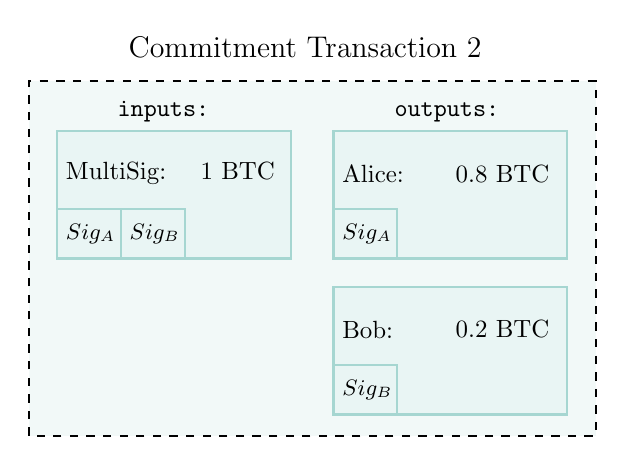
\begin{tikzpicture}[scale=0.9, every node/.style={scale=0.9}]
					\filldraw[yshift=-0.05cm, xshift=0.1cm,color = highlight!15, thick, 	draw=black, dashed] (-3,-5.9) rectangle ++(8cm,5cm);

\draw[color=black] plot (1,-0.2) node [below]
{\large{{Commitment Transaction 2}}};

% Inputs
\draw[color=black] plot (-1,-1.65) node[above] {\texttt{inputs:}};

% top left
\filldraw[yshift=-0.05cm, xshift=0.1cm,color = highlight!25, thick, 	draw=highlight] (-2.6,-3.4) rectangle ++(3.3cm,1.8cm);
\filldraw[yshift=-0.05cm, xshift=0.1cm,color = highlight!25, thick, 	draw=highlight] (-2.6,-3.4) rectangle ++(0.9cm,0.7cm);
\filldraw[yshift=-0.05cm, xshift=0.1cm,color = highlight!25, thick, 	draw=highlight] (-1.7,-3.4) rectangle ++(0.9cm,0.7cm);
\draw[color=black] plot (-2.5,-2.25) node[right] {MultiSig:};
\draw[color=black] plot (-0.6,-2.21)   node[right] {1 BTC};
\draw[color=black] plot (-2.5,-3.1)   node[right] {\small{$Sig_A$}};
\draw[color=black] plot (-1.6,-3.1)   node[right] {\small{$Sig_B$}};

\draw plot (-2,-3.1) node {\checkmarkgreen};
\uncover<3->{\draw plot (-1.1,-3.1) node {\checkmarkgreen};}

% Outputs
\draw[color=black] plot (3,-1.65)   node[above] {\texttt{outputs:}};

% top right
\filldraw[yshift=-0.05cm, xshift=0.1cm,color = highlight!25, thick, draw=highlight] (1.3,-3.4) rectangle ++(3.3cm,1.8cm);
\filldraw[yshift=-0.05cm, xshift=0.1cm,color = highlight!25, thick, 	draw=highlight] (1.3,-3.4) rectangle ++(0.9cm,0.7cm);
\draw[color=black] plot (1.4,-2.25)   node[right] {Alice:};
\draw[color=black] plot (3,-2.25)   node[right] {0.8 BTC};
\draw[color=black] plot (1.4,-3.1)   node[right] {\small{$Sig_A$}};

% bottom right
\filldraw[yshift=-0.05cm, xshift=0.1cm,color = highlight!25, thick, draw=highlight] (1.3,-5.6) rectangle ++(3.3cm,1.8cm);
\filldraw[yshift=-0.05cm, xshift=0.1cm,color = highlight!25, thick,draw=highlight] (1.3,-5.6) rectangle ++(0.9cm,0.7cm);
\draw[color=black] plot (1.4,-4.45)   node[right] {Bob:};
\draw[color=black] plot (3,-4.45)   node[right] {0.2 BTC};
\draw[color=black] plot (1.4,-5.3)   node[right] {\small{$Sig_B$}};
			\end{tikzpicture}}
		\end{figure}}		
	\end{minipage}%
	\begin{minipage}{0.1\linewidth}
		\vspace{1.44cm}
		\centering
		
\includegraphics[width=1cm]{../assets/images/agents/handing_left}
		\\ \hspace{0.3cm}\textbf{Bob}
		\vspace{-0.5cm}
		\begin{figure}
		\hspace{-1.7cm}
		\resizebox{2.5cm}{!}{
				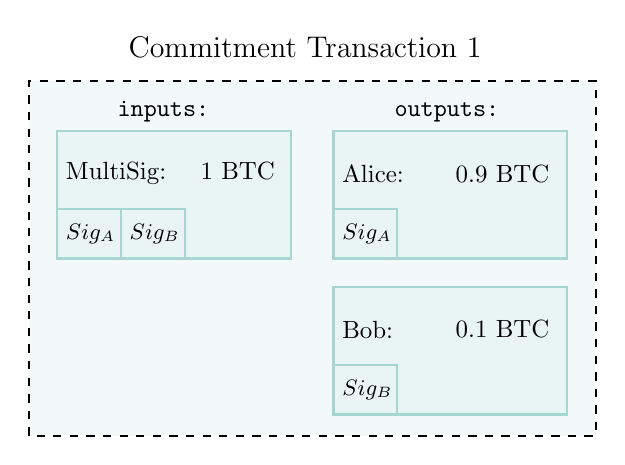
\begin{tikzpicture}[scale=0.9, every node/.style={scale=0.9}]
						\filldraw[yshift=-0.05cm, xshift=0.1cm,color = highlight!15, thick, 	draw=black, dashed] (-3,-5.9) rectangle ++(8cm,5cm);
	
	\draw[color=black] plot (1,-0.2) node [below]
	{\large{{Commitment Transaction 1}}};
	
	% Inputs
	\draw[color=black] plot (-1,-1.65) node[above] {\texttt{inputs:}};
	
	% top left
	\filldraw[yshift=-0.05cm, xshift=0.1cm,color = highlight!25, thick, 	draw=highlight] (-2.6,-3.4) rectangle ++(3.3cm,1.8cm);
	\filldraw[yshift=-0.05cm, xshift=0.1cm,color = highlight!25, thick, 	draw=highlight] (-2.6,-3.4) rectangle ++(0.9cm,0.7cm);
	\filldraw[yshift=-0.05cm, xshift=0.1cm,color = highlight!25, thick, 	draw=highlight] (-1.7,-3.4) rectangle ++(0.9cm,0.7cm);
	\draw[color=black] plot (-2.5,-2.25) node[right] {MultiSig:};
	\draw[color=black] plot (-0.6,-2.21)   node[right] {1 BTC};
	\draw[color=black] plot (-2.5,-3.1)   node[right] {\small{$Sig_A$}};
	\draw[color=black] plot (-1.6,-3.1)   node[right] {\small{$Sig_B$}};
	
	\draw plot (-2,-3.1) node {\checkmarkgreen};
	
	% Outputs
	\draw[color=black] plot (3,-1.65)   node[above] {\texttt{outputs:}};
	
	% top right
	\filldraw[yshift=-0.05cm, xshift=0.1cm,color = highlight!25, thick, draw=highlight] (1.3,-3.4) rectangle ++(3.3cm,1.8cm);
	\filldraw[yshift=-0.05cm, xshift=0.1cm,color = highlight!25, thick, 	draw=highlight] (1.3,-3.4) rectangle ++(0.9cm,0.7cm);
	\draw[color=black] plot (1.4,-2.25)   node[right] {Alice:};
	\draw[color=black] plot (3,-2.25)   node[right] {0.9 BTC};
	\draw[color=black] plot (1.4,-3.1)   node[right] {\small{$Sig_A$}};
	
	% bottom right
	\filldraw[yshift=-0.05cm, xshift=0.1cm,color = highlight!25, thick, draw=highlight] (1.3,-5.6) rectangle ++(3.3cm,1.8cm);
	\filldraw[yshift=-0.05cm, xshift=0.1cm,color = highlight!25, thick,draw=highlight] (1.3,-5.6) rectangle ++(0.9cm,0.7cm);
	\draw[color=black] plot (1.4,-4.45)   node[right] {Bob:};
	\draw[color=black] plot (3,-4.45)   node[right] {0.1 BTC};
	\draw[color=black] plot (1.4,-5.3)   node[right] {\small{$Sig_B$}};

				\end{tikzpicture}}
		\end{figure}
	\end{minipage}
\end{frame}

%%%
\begin{frame}{UPC: Incentives & Role of Timelocks}


\end{frame}
%%%


%%%
\begin{frame}{Bidirectional Payment Channel (BPC): Setup}




\end{frame}
%%%


%%%
\begin{frame}{BPC: Incentives & Role of Timelocks}


\end{frame}
%%%


%%%
\begin{frame}{Channels with Asymmetric Revocable Commitments (CwARC)}


\end{frame}
%%%


%%%
\begin{frame}{Challenges with Payment Channels}


\end{frame}
%%%

%%%
\begin{frame}{Lightning Network Approach (simplified)}


\end{frame}
%%%

%%%
\begin{frame}{Lightning Network Implications}


\end{frame}
%%%

%%%
\begin{frame}{SUPC: Setup Transactions}
	
%%%
\begin{frame}{SUPC: First Payment}
	
\end{frame}
%%%




%%%

\begin{frame}{Bib-References}
		Read the Bitcoin Whitepaper, \cite{nakamotoBitcoin2008}.
\end{frame}


\begin{frame}%[allowframebreaks]
\frametitle{References and Recommended Reading}
	\bibliographystyle{amsplain}
	\bibliography{../assets/bib/refs}
\end{frame}


\end{document}